\documentclass[12pt,a4paper]{article}

% ---- Fonts & encoding ----
% XeLaTeX configuration for Armenian
\usepackage{fontspec}
\setmainfont{Sylfaen} % Standard Windows font with Armenian support
\setsansfont{Arial}
\usepackage{microtype}
\newcommand{\armtext}{} % Defined as empty for XeLaTeX workflow

% ---- Layout ----
\usepackage[margin=1in, headheight=15pt]{geometry}

% ---- Core math ----
\usepackage{amsmath,amssymb,amsthm}
\usepackage{mathtools}
\usepackage{enumitem}

% ---- Visual ----
\usepackage[dvipsnames,svgnames]{xcolor}
\usepackage[framemethod=tikz]{mdframed}
\usepackage{tikz}
  \usetikzlibrary{calc,arrows.meta,decorations.pathreplacing,positioning,shapes.geometric}
\usepackage{booktabs}
\usepackage{fancyhdr}
\usepackage{titlesec}
\usepackage[bookmarksnumbered]{hyperref}
\usepackage{bookmark}

% ---- Colour palette ----
\definecolor{ProbBG}{HTML}{EAF0F9}
\definecolor{ProbFrame}{HTML}{3360A0}
\definecolor{SolBG}{HTML}{F6F8F4}
\definecolor{SolFrame}{HTML}{4A8C5C}
\definecolor{AccGold}{HTML}{C5960C}
\definecolor{SectCol}{HTML}{22406A}
\definecolor{GridGray}{HTML}{D0D0D0}

% ---- Page style ----
\pagestyle{fancy}
\fancyhf{}
\renewcommand{\headrulewidth}{0.6pt}
\renewcommand{\headrule}{\hbox to\headwidth{%
  \color{SectCol}\leaders\hrule height \headrulewidth\hfill}}
\fancyhead[L]{\color{SectCol}\textsc{\armtext{Խմբերի տեսություն}}}
\fancyhead[R]{\color{SectCol}\textsc{\armtext{Գործնական 10}}}
\fancyfoot[C]{\color{SectCol}\thepage}

% ---- Section formatting ----
\titleformat{\section}
  {\color{SectCol}\large\bfseries}
  {\fcolorbox{SectCol}{SectCol}{\color{white}\;\thesection\;}}{0.6em}{}
  [\vspace{-0.3em}\color{SectCol}\titlerule]
\titleformat{\subsection}
  {\color{SectCol}\normalsize\bfseries}
  {\thesubsection.}{0.5em}{}

% ---- mdframed: problem statement ----
\mdfdefinestyle{problemstyle}{
  linewidth=0.8pt,
  linecolor=ProbFrame,
  backgroundcolor=ProbBG,
  roundcorner=3pt,
  innertopmargin=8pt,
  innerbottommargin=8pt,
  innerleftmargin=10pt,
  innerrightmargin=10pt,
  font=\itshape
}
\newenvironment{problem}{\begin{mdframed}[style=problemstyle]\armtext}{\end{mdframed}}

% ---- mdframed: solution ----
\mdfdefinestyle{solstyle}{
  linewidth=0.6pt,
  linecolor=SolFrame,
  backgroundcolor=SolBG,
  roundcorner=3pt,
  innertopmargin=8pt,
  innerbottommargin=8pt,
  innerleftmargin=10pt,
  innerrightmargin=10pt,
  frametitle={\colorbox{SolFrame}{\color{white}\;\textbf{\sffamily \armtext{Լուծում}}\;}},
  frametitleaboveskip=-\ht\strutbox,
  frametitlealignment=\raggedright
}
\newenvironment{sol}{\begin{mdframed}[style=solstyle]\armtext}{\end{mdframed}}

% ---- Math shortcuts ----
\newcommand{\Z}{\mathbb{Z}}
\newcommand{\Q}{\mathbb{Q}}
\newcommand{\R}{\mathbb{R}}
\newcommand{\C}{\mathbb{C}}
\newcommand{\N}{\mathbb{N}}
\newcommand{\Rstar}{\mathbb{R}^{*}}
\newcommand{\Cstar}{\mathbb{C}^{*}}
\newcommand{\Rplus}{\mathbb{R}_{>0}}
\newcommand{\abs}[1]{\left|#1\right|}
\newcommand{\gen}[1]{\langle #1 \rangle}
\newcommand{\normal}{\trianglelefteq}
\DeclareMathOperator{\ord}{ord}
\DeclareMathOperator{\lcm}{lcm}
\DeclareMathOperator{\Ker}{Ker}
\DeclareMathOperator{\im}{Im}
\DeclareMathOperator{\Aut}{Aut}
\DeclareMathOperator{\Inn}{Inn}
\DeclareMathOperator{\id}{id}
\DeclareMathOperator{\Cent}{Z}
\DeclareMathOperator{\sgn}{sgn}

% ===========================================================================
\begin{document}
% ===========================================================================

% ---- Title ----
\begin{mdframed}[
  linewidth=0pt,
  backgroundcolor=SectCol,
  roundcorner=4pt,
  innertopmargin=14pt,
  innerbottommargin=14pt,
  font=\color{white}\centering
]
  {\fontsize{22}{26}\selectfont\bfseries\sffamily \armtext{Գործնական 10}}\\[8pt]
  {\large\sffamily \armtext{Խմբերի ուղիղ արտադրյալներ և վերլուծություններ}}\\[6pt]
  {\color{white!70!SectCol}\rule{5cm}{0.4pt}}
\end{mdframed}

\vspace{1.2em}

%==========================================================================
\section{\armtext{Կլեյնի խումբը որպես ուղիղ արտադրյալ}}
%==========================================================================

\begin{problem}
Ցույց տալ, որ Կլեյնի $V_4$ խումբը կարող է վերլուծվել երկու երկրորդ կարգի ցիկլիկ խմբերի ուղիղ արտադրյալի:
\end{problem}

\begin{sol}
Հիշենք, որ Կլեյնի խումբը $V_4 = \{e,\, a,\, b,\, c\}$ խումբն է, որտեղ յուրաքանչյուր ոչ միավոր տարր ունի 2 կարգ, և բազմապատկումը տրվում է $ab = c$, $ac = b$, $bc = a$ առնչություններով:

\medskip
\begin{center}
\begin{tikzpicture}[every node/.style={font=\small}]
  % Cayley table header
  \node[font=\small\bfseries] at (0,0) {$\cdot$};
  \foreach \j/\el in {1/e, 2/a, 3/b, 4/c}{
    \node[font=\small\bfseries, text=ProbFrame] at (\j*1.1, 0) {$\el$};
    \node[font=\small\bfseries, text=ProbFrame] at (0, -\j*0.7) {$\el$};
  }
  % Row 1: e*e, e*a, e*b, e*c
  \node at (1.1,-0.7) {$e$}; \node at (2.2,-0.7) {$a$};
  \node at (3.3,-0.7) {$b$}; \node at (4.4,-0.7) {$c$};
  % Row 2: a*e, a*a, a*b, a*c
  \node at (1.1,-1.4) {$a$}; \node at (2.2,-1.4) {$e$};
  \node at (3.3,-1.4) {$c$}; \node at (4.4,-1.4) {$b$};
  % Row 3: b*e, b*a, b*b, b*c
  \node at (1.1,-2.1) {$b$}; \node at (2.2,-2.1) {$c$};
  \node at (3.3,-2.1) {$e$}; \node at (4.4,-2.1) {$a$};
  % Row 4: c*e, c*a, c*b, c*c
  \node at (1.1,-2.8) {$c$}; \node at (2.2,-2.8) {$b$};
  \node at (3.3,-2.8) {$a$}; \node at (4.4,-2.8) {$e$};
  % Dividers
  \draw[ProbFrame, thick] (0.55,0.35) -- (0.55,-3.15);
  \draw[ProbFrame, thick] (-0.55,-0.35) -- (5.05,-0.35);
  \node[anchor=north, font=\footnotesize\sffamily, text=SectCol] at (2.2,-3.5)
    {\armtext{$V_4$-ի Քելիի աղյուսակը}};
\end{tikzpicture}
\end{center}

Դիտարկենք ենթախմբերը՝
\[
  H = \gen{a} = \{e, a\} \cong \Z_2, \qquad
  K = \gen{b} = \{e, b\} \cong \Z_2.
\]

Ստուգենք $V_4 = H \times K$ \emph{ներքին} ուղիղ արտադրյալի երեք պայմանները.

\begin{enumerate}[label=\textcolor{SolFrame}{(\roman*)},leftmargin=*]
  \item \textbf{$H$-ը և $K$-ն նորմալ են $V_4$-ում:}
    Քանի որ $V_4$-ը աբելյան է, յուրաքանչյուր ենթախումբ նորմալ է:

  \item \textbf{$H \cap K = \{e\}$.}
    $\{e,a\}$ և $\{e,b\}$ խմբերի միակ ընդհանուր տարրը $e$-ն է:

  \item \textbf{$HK = V_4$.}
    $HK = \{e \cdot e,\; e \cdot b,\; a \cdot e,\; a \cdot b\}
         = \{e,\, b,\, a,\, c\} = V_4.$
\end{enumerate}

Հետևաբար $V_4 = H \times K \cong \Z_2 \times \Z_2$: \qed
\end{sol}

\bigskip
%==========================================================================
\section{\armtext{$S_3$, $A_4$ և $S_4$ խմբերի վերլուծելիությունը}}
%==========================================================================

\begin{problem}
Արդյոք $S_{3},$ $A_{4}$ և $S_{4}$ խմբերը վերլուծելի են (ոչ տրիվիալ) ենթախմբերի ուղիղ արտադրյալի:
\end{problem}

\begin{sol}
\textbf{\color{SectCol}$S_3$-ը անվերլուծելի է:}\;
$|S_3| = 6$: Ոչ տրիվիալ վերլուծության համար պետք է $S_3 \cong H \times K$, որտեղ
$|H|=2$, $|K|=3$: Այդ դեպքում $H \times K \cong \Z_2 \times \Z_3 \cong \Z_6$-ը
աբելյան է, բայց $S_3$-ը ոչ աբելյան է: Հակասություն:

\medskip
\textbf{\color{SectCol}$A_4$-ը անվերլուծելի է:}\;
$|A_4|=12$: Հնարավոր ենթախմբերի կարգերը՝ $(2,6)$, $(3,4)$, $(2,2,3)$:

\begin{itemize}[leftmargin=*]
  \item \textbf{$(2,6)$:} $A_4$-ը ընդհանրապես չունի 6-րդ կարգի ենթախումբ
    ($A_4$-ը ամենափոքր խումբն է, որտեղ $6 \mid |G|$, բայց չկա 6-րդ կարգի ենթախումբ):

  \item \textbf{$(3,4)$:} Կլեյնի չորրորդ կարգի խումբը
    $V = \{e, (12)(34), (13)(24), (14)(23)\} \normal A_4$
    ունի 4 կարգ, իսկ $\gen{(123)}$-ը՝ 3 կարգ, ընդ որում
    $V \cap \gen{(123)} = \{e\}$: Սակայն $\gen{(123)}$-ը
    \emph{նորմալ չէ} $A_4$-ում (օրինակ՝
    $(12)(34)(123)(12)(34) = (243) \notin \gen{(123)}$):

  \item \textbf{$(2,2,3)$:} $A_4$-ը ունի միայն մեկ 4-րդ կարգի ենթախումբ,
    ուստի հնարավոր չէ գտնել պահանջվող 2-րդ կարգի նորմալ ենթախմբերի զույգը:
\end{itemize}

\begin{center}
\begin{tikzpicture}[
  every node/.style={font=\small},
  nd/.style={draw, rounded corners=2pt, fill=ProbBG, inner sep=3pt,
             minimum width=1.2cm, font=\small},
  >=Stealth]
  \node[nd] (A4) at (0,3) {$A_4$};
  \node[nd] (V)  at (-2.5,1.5) {$V_4$};
  \node[nd] (H1) at (-0.2,1.5) {$\gen{(123)}$};
  \node[nd] (H2) at (1.8,1.5) {$\gen{(124)}$};
  \node[nd,draw=none,fill=none] at (3.3,1.5) {$\cdots$};
  \node[nd] (e)  at (0,0) {$\{e\}$};
  \draw[thick,ProbFrame] (A4)--(V)--(e) (A4)--(H1)--(e) (A4)--(H2)--(e);
  \node[anchor=north,font=\footnotesize\sffamily,text=SectCol] at (0,-0.6)
    {\armtext{$A_4$-ի ենթախմբերի ցանցը (մասնակի) - չկա համապատասխան զույգ}};
\end{tikzpicture}
\end{center}

\textbf{\color{SectCol}$S_4$-ը անվերլուծելի է:}\;
$|S_4|=24$: Միակ սեփական ոչ տրիվիալ նորմալ ենթախմբերն են $A_4$-ը (կարգը՝ 12)
և $V_4$-ը (կարգը՝ 4):
\begin{itemize}[leftmargin=*]
  \item $H = A_4$, $|K|=2$: գոյություն չունի 2-րդ կարգի նորմալ ենթախումբ:
  \item $H = V_4$, $|K|=6$: գոյություն չունի 6-րդ կարգի նորմալ ենթախումբ:
\end{itemize}

Բոլոր երեք խմբերը \textbf{անվերլուծելի} են: \qed
\end{sol}

\bigskip
%==========================================================================
\section{\armtext{$\Z$-ը և $\Q$-ն անվերլուծելի են (ադիտիվ)}}
%==========================================================================

\begin{problem}
Ապացուցել, որ $\Z$ և $\Q$ ադիտիվ խմբերը չեն կարող վերլուծվել այնպիսի ենթախմբերի ուղիղ գումարի, որոնցից ոչ մեկը զրոյական չէ:
\end{problem}

\begin{sol}
\textbf{\color{SectCol}Դեպք $\Z$:}\;
Ենթադրենք $\Z = A \oplus B$, որտեղ $A, B \neq 0$:
$\Z$-ի յուրաքանչյուր ոչ տրիվիալ ենթախումբ ունի $n\Z$ տեսքը, ուստի $A = m\Z$, $B = n\Z$,
որտեղ $m, n \geq 1$:

\begin{itemize}[leftmargin=*]
  \item $A + B = \Z \implies \gcd(m,n)=1$\; (հակառակ դեպքում $m\Z + n\Z$-ի յուրաքանչյուր տարր
    բաժանվում է $\gcd(m,n) > 1$-ի):
  \item $A \cap B = m\Z \cap n\Z = \lcm(m,n)\Z = mn\Z$\; (քանի որ $\gcd(m,n)=1$):
\end{itemize}

$A \cap B = \{0\}$ պայմանի համար պետք է $mn = 0$, ինչը անհնար է $m,n \geq 1$ դեպքում: Հակասություն:

\begin{center}
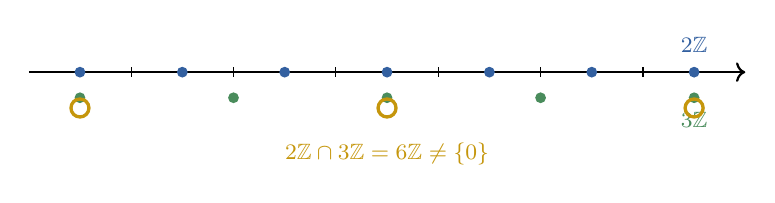
\begin{tikzpicture}[scale=0.65]
  \draw[->,thick] (-7,0) -- (7,0);
  \foreach \x in {-6,...,6}
    \draw (\x,0.1)--(\x,-0.1);
  % 2Z
  \foreach \x in {-6,-4,-2,0,2,4,6}
    \fill[ProbFrame] (\x,0) circle (3pt);
  \node[font=\footnotesize,text=ProbFrame,above] at (6,0.2) {$2\Z$};
  % 3Z
  \foreach \x in {-6,-3,0,3,6}
    \fill[SolFrame] (\x,-0.5) circle (3pt);
  \node[font=\footnotesize,text=SolFrame,below] at (6,-0.6) {$3\Z$};
  % overlap
  \foreach \x in {-6,0,6}
    \draw[AccGold,very thick] (\x,-0.7) circle (5pt);
  \node[font=\footnotesize\sffamily,text=AccGold,below] at (0,-1.2)
    {$2\Z \cap 3\Z = 6\Z \neq \{0\}$};
\end{tikzpicture}
\end{center}

\textbf{\color{SectCol}Դեպք $\Q$:}\;
Ենթադրենք $\Q = A \oplus B$, որտեղ $A, B \neq 0$:
Ընտրենք $0 \neq a \in A$ և $0 \neq b \in B$:
Գրենք նրանց ընդհանուր հայտարարով՝ $a = \alpha/d$, $b = \beta/d$,
որտեղ $\alpha, \beta, d \in \Z$, $d > 0$:

Քանի որ $A$-ն ենթախումբ է, որը պարունակում է $a = \alpha/d$, այն պարունակում է նաև
$\beta \cdot a = \alpha\beta/d$: Նմանապես $B$-ն պարունակում է
$\alpha \cdot b = \alpha\beta/d$:

Ուստի $\alpha\beta/d \in A \cap B$, ընդ որում $\alpha\beta/d \neq 0$
(քանի որ $\alpha, \beta \neq 0$),
ինչը հակասում է $A \cap B = \{0\}$ պայմանին: \qed
\end{sol}

\bigskip
%==========================================================================
\section{\armtext{$(\C,+)$ և $(\Cstar, \cdot)$ խմբերի վերլուծությունները}}
%==========================================================================

\subsection{$(\C,+) \cong (\R,+) \oplus (\R,+)$}

\begin{problem}
Ապացուցել, որ կոմպլեքս թվերի ադիտիվ խումբը կարող է վերլուծվել իրական և կեղծ թվերի ադիտիվ խմբերի ուղիղ գումարի:
\end{problem}

\begin{sol}
Դիցուք $A = \R$ և $B = i\R = \{bi : b \in \R\}$, երկուսն էլ $(\C,+)$-ի ենթախմբեր են:

\begin{enumerate}[label=\textcolor{SolFrame}{(\roman*)},leftmargin=*]
  \item \textbf{Նորմալություն:} $(\C,+)$-ը աբելյան է, ուստի բոլոր ենթախմբերը նորմալ են:
  \item \textbf{$A \cap B = \{0\}$.}
    $z \in A \cap B$ $\Rightarrow$ $z$-ը և՛ իրական է, և՛ կեղծ $\Rightarrow$ $z=0$:
  \item \textbf{$A + B = \C$.}
    Յուրաքանչյուր $z \in \C$ ներկայացվում է $z = \underbrace{\Re(z)}_{\in\, A}
    + \underbrace{i\,\Im(z)}_{\in\, B}$ տեսքով:
\end{enumerate}

\begin{center}
\begin{tikzpicture}[scale=0.75]
  \draw[->,thick,gray!60] (-3.2,0)--(3.2,0) node[right,font=\small]{$\R$};
  \draw[->,thick,gray!60] (0,-2.7)--(0,2.7) node[above,font=\small]{$i\R$};
  \coordinate (P) at (2,1.6);
  \fill[AccGold] (P) circle (3pt);
  \node[font=\small,above right] at (P) {$z = x + iy$};
  \draw[dashed, ProbFrame, thick] (P) -- (2,0);
  \draw[dashed, SolFrame,  thick] (P) -- (0,1.6);
  \fill[ProbFrame] (2,0) circle (2.5pt);
  \fill[SolFrame]  (0,1.6) circle (2.5pt);
  \node[font=\footnotesize, ProbFrame, below] at (2,0) {$x \in A$};
  \node[font=\footnotesize, SolFrame, left]  at (0,1.6) {$iy \in B$};
  \node[font=\footnotesize\sffamily, SectCol, anchor=north] at (0,-3.1)
    {\armtext{Ամեն $z\in\C$ միակորեն ներկայացվում է $z = x + iy$}};
\end{tikzpicture}
\end{center}

Հետևաբար $(\C,+) = A \oplus B \cong (\R,+) \oplus (\R,+)$: \qed
\end{sol}

\subsection{$(\Cstar, \cdot) \cong (\Rplus, \cdot) \times (S^1, \cdot)$}

\begin{problem}
Ապացուցել, որ ոչ զրոյական կոմպլեքս թվերի բազմապատկական խումբը կարող է վերլուծվել դրական իրական թվերի և մոդուլով մեկ կոմպլեքս թվերի խմբերի ուղիղ արտադրյալի:
\end{problem}

\begin{sol}
Դիցուք $P = \Rplus$ (դրական իրական թվերը բազմապատկումով) և
$S^1 = \{z \in \C : |z|=1\}$ (միավոր շրջանագիծ):

\begin{enumerate}[label=\textcolor{SolFrame}{(\roman*)},leftmargin=*]
  \item \textbf{Նորմալություն:} $\Cstar$-ը աբելյան է:
  \item \textbf{$P \cap S^1 = \{1\}$.}
    $r \in P \cap S^1 \Rightarrow r > 0$ և $|r|=1 \Rightarrow r=1$:
  \item \textbf{$P \cdot S^1 = \Cstar$.}
    Յուրաքանչյուր $z \neq 0$ գրվում է
    $z = \underbrace{|z|}_{\in\, P}\;\cdot\;\underbrace{z/|z|}_{\in\, S^1}$ տեսքով:
\end{enumerate}

\begin{center}
\begin{tikzpicture}[scale=0.85]
  \draw[->,thick,gray!50] (-2.5,0)--(3.5,0);
  \draw[->,thick,gray!50] (0,-2.2)--(0,2.5);
  \draw[SolFrame, thick] (0,0) circle (1);
  \node[font=\footnotesize, SolFrame] at (1.35,0.85) {$S^1$};
  \coordinate (P) at (55:2.3);
  \draw[ProbFrame, thick, dashed] (0,0) -- (55:3);
  \fill[AccGold] (P) circle (3pt);
  \node[font=\small, above right] at (P) {$z$};
  \coordinate (U) at (55:1);
  \fill[SolFrame] (U) circle (2.5pt);
  \node[font=\footnotesize, SolFrame, below left] at (U) {$\frac{z}{|z|}$};
  \draw[<->,ProbFrame, thick] (0,-0.15) -- node[below,font=\footnotesize]{$|z|$}
    ($(55:2.3)+(0,-0.15)$);
  \node[font=\footnotesize\sffamily, SectCol, anchor=north] at (0.5,-2.6)
    {\armtext{Բևեռային վերլուծություն. $z = |z| \cdot e^{i\theta}$}};
\end{tikzpicture}
\end{center}

Հետևաբար $(\Cstar, \cdot) = P \times S^1 \cong (\Rplus, \cdot) \times (S^1, \cdot)$: \qed
\end{sol}

\bigskip
%==========================================================================
\section{\armtext{Քվատերնիոնների խումբը անվերլուծելի է}}
%==========================================================================

\begin{problem}
Ապացուցել, որ $Q_8$ քվատերնիոնների խումբը անվերլուծելի է:
\end{problem}

\begin{sol}
Հիշենք, որ $Q_8 = \{\pm 1, \pm i, \pm j, \pm k\}$, $|Q_8|=8$:
Ոչ տրիվիալ վերլուծության համար անհրաժեշտ է $(|H|,|K|) \in \{(2,4),(4,2)\}$:

\textbf{$Q_8$-ի ենթախմբերը:}

\begin{center}
\begin{tikzpicture}[
  nd/.style={draw, rounded corners=2pt, fill=ProbBG, inner sep=3pt,
             font=\small, minimum width=1.6cm},
  >=Stealth]
  \node[nd,fill=ProbFrame!15] (Q) at (0,3.5) {$Q_8$};
  \node[nd] (I) at (-3,2)   {$\gen{i}$};
  \node[nd] (J) at ( 0,2)   {$\gen{j}$};
  \node[nd] (K) at ( 3,2)   {$\gen{k}$};
  \node[nd,fill=AccGold!20] (C) at (0,0.5) {$\{1,-1\}$};
  \node[nd] (E) at (0,-0.8) {$\{1\}$};
  \draw[thick] (Q)--(I)--(C) (Q)--(J)--(C) (Q)--(K)--(C) (C)--(E);
  % annotation
  \draw[AccGold, very thick, rounded corners=3pt]
    (-1.1,0.1) rectangle (1.1,0.95);
  \node[font=\footnotesize\sffamily, AccGold, anchor=west] at (1.3,0.5)
    {\armtext{միակ 2-րդ կարգի ենթախումբը}};
  % side labels
  \node[font=\scriptsize, gray, right] at (3.8,2) {$= \{\pm 1, \pm k\}$};
  \node[font=\scriptsize, gray, left]  at (-3.8,2) {$= \{\pm 1, \pm i\}$};
  \node[font=\scriptsize, gray, right] at (0.8,2) {$= \{\pm 1, \pm j\}$};
\end{tikzpicture}
\end{center}

Գոյություն ունի ճիշտ \emph{մեկ} ենթախումբ 2 կարգի՝ կենտրոնը $\{1,-1\}$:
Յուրաքանչյուր 4-րդ կարգի ենթախումբ պարունակում է $-1$-ը, հետևաբար պարունակում է $\{1,-1\}$:

Ցանկացած $Q_8 = H \times K$ փորձի համար, որտեղ $|H|=2$, $|K|=4$.
\[
  H = \{1,-1\}, \quad K \in \bigl\{\gen{i},\,\gen{j},\,\gen{k}\bigr\}
  \quad\Longrightarrow\quad
  H \cap K \supseteq \{1,-1\} \neq \{1\}.
\]

Սա խախտում է $H \cap K = \{1\}$ պայմանը, ուստի $Q_8$-ը անվերլուծելի է: \qed
\end{sol}

\bigskip
%==========================================================================
\section{\armtext{$\Rstar$-ը վերլուծելի է}}
%==========================================================================

\begin{problem}
Ապացուցել, որ $\Rstar$ խումբը (ոչ զրոյական իրական թվերը բազմապատկումով) վերլուծելի է:
\end{problem}

\begin{sol}
Դիցուք $P = \Rplus = \{x \in \R : x > 0\}$ և $N = \{1,-1\} \cong \Z_2$:

\begin{enumerate}[label=\textcolor{SolFrame}{(\roman*)},leftmargin=*]
  \item \textbf{Նորմալություն:} $\Rstar$-ը աբելյան է:
  \item \textbf{$P \cap N = \{1\}$.} $\{1,-1\}$ բազմության միակ դրական տարրը $1$-ն է:
  \item \textbf{$PN = \Rstar$.}
    Յուրաքանչյուր $x \neq 0$ գրվում է $x = |x| \cdot \sgn(x)$ տեսքով, որտեղ $|x| \in P$, $\sgn(x) \in N$:
\end{enumerate}

\begin{center}
\begin{tikzpicture}[scale=0.8]
  \draw[->,thick,gray!50] (-5,0)--(5,0);
  \fill[ProbFrame!20] (0.05,-0.4) rectangle (4.8,0.4);
  \fill[SolFrame!20]  (-4.8,-0.4) rectangle (-0.05,0.4);
  \node[font=\footnotesize,ProbFrame] at (2.5,0.7) {$P = \Rplus$};
  \node[font=\footnotesize,SolFrame] at (-2.5,0.7) {$(-1)\cdot P$};
  \fill[AccGold] (0,0) circle (2.5pt);
  \node[font=\footnotesize,below,AccGold] at (0,-0.55) {$0$ \armtext{(բացառված)}};
  \draw[thick,decorate,decoration={brace,amplitude=4pt,mirror}]
    (-4.8,-0.7) -- (4.8,-0.7)
    node[midway,below=5pt,font=\footnotesize\sffamily,SectCol]
    {$\Rstar = P \times \{1,-1\} \;\cong\; \Rplus \times \Z_2$};
\end{tikzpicture}
\end{center}
\qed
\end{sol}

\bigskip
%==========================================================================
\section{\armtext{Ուղիղ արտադրյալի կենտրոնը}}
%==========================================================================

\begin{problem}
Ապացուցել, որ $\Cent(G \times H) = \Cent(G) \times \Cent(H)$:
\end{problem}

\begin{sol}
\noindent$(\subseteq)$\;
Դիցուք $(g,h) \in \Cent(G \times H)$:
Յուրաքանչյուր $(x,y) \in G \times H$ տարրի համար.
\[
  (g,h)(x,y) = (x,y)(g,h)
  \;\Longrightarrow\;
  \begin{cases} gx = xg & \forall\, x \in G,\\[2pt] hy = yh & \forall\, y \in H, \end{cases}
\]
ուստի $g \in \Cent(G)$ և $h \in \Cent(H)$:

\medskip
\noindent$(\supseteq)$\;
Եթե $g \in \Cent(G)$ և $h \in \Cent(H)$, ապա ամեն $(x,y)$-ի համար.
\[
  (g,h)(x,y) = (gx,hy) = (xg,yh) = (x,y)(g,h).
\]

Ինդուկցիայով՝ $\displaystyle\Cent\!\Bigl(\prod_{i=1}^{n} G_i\Bigr) = \prod_{i=1}^{n} \Cent(G_i).$ \qed
\end{sol}

\bigskip
%==========================================================================
\section{\armtext{Ուղիղ արտադրյալի կոմուտանտը}}
%==========================================================================

\begin{problem}
Ապացուցել, որ $[G \times H,\, G \times H] = [G,G] \times [H,H]$:
\end{problem}

\begin{sol}
\noindent$(\supseteq)$\;
$[g_1,g_2] \in [G,G]$-ի համար.
\[
  \bigl([g_1,g_2],\, e_H\bigr)
  = \bigl[(g_1,e_H),\,(g_2,e_H)\bigr]
  \in [G \times H,\, G \times H].
\]
Նույնը $[H,H]$-ի համար: Քանի որ $[G\times H, G\times H]$-ը ենթախումբ է, այն
պարունակում է $[G,G] \times [H,H]$-ը:

\medskip
\noindent$(\subseteq)$\;
Ամեն կոմուտատոր գործոնավորվում է ըստ բաղադրիչների.
\[
  [(g_1,h_1),\,(g_2,h_2)]
  = \bigl(g_1^{-1}g_2^{-1}g_1 g_2,\;\; h_1^{-1}h_2^{-1}h_1 h_2\bigr)
  = \bigl([g_1,g_2],\;[h_1,h_2]\bigr)
  \in [G,G] \times [H,H].
\]
Քանի որ $[G \times H, G \times H]$-ը ծնվում է նման կոմուտատորներով, հետևում է պարփակումը: \qed
\end{sol}

\bigskip
%==========================================================================
\section{\armtext{385 կարգի աբելյան խումբ}}
%==========================================================================

\begin{problem}
Ապացուցել, որ 385 կարգի աբելյան խումբը կարող է վերլուծվել 5, 7 և 11 կարգի ցիկլիկ ենթախմբերի ուղիղ գումարի:
\end{problem}

\begin{sol}
$385 = 5 \times 7 \times 11$ (քառակուսազուրկ):

\textbf{Ըստ հիմնական թեորեմի.}\;
Քանի որ յուրաքանչյուր պարզ թիվ մասնակցում է միայն առաջին աստիճանով, միակ վերլուծությունն է.
\[
  G \cong \Z_5 \oplus \Z_7 \oplus \Z_{11} \cong \Z_{385}.
\]

\textbf{Տարրական ապացույց.}\;
Ըստ Կոշիի թեորեմի, ընտրենք $a,b,c$ տարրեր $5,7,11$ կարգերով:
Դիցուք $A = \gen{a}$, $B = \gen{b}$, $C = \gen{c}$:

\begin{center}
\begin{tikzpicture}[every node/.style={font=\small}]
  \node[draw, circle, minimum size=1.4cm, thick, ProbFrame, fill=ProbBG]
    (A) at (0,0) {$\gen{a}$};
  \node[font=\scriptsize,ProbFrame] at (0,-1.1) {\armtext{կարգը 5}};
  \node[draw, circle, minimum size=1.4cm, thick, SolFrame, fill=SolBG]
    (B) at (2.6,0) {$\gen{b}$};
  \node[font=\scriptsize,SolFrame] at (2.6,-1.1) {\armtext{կարգը 7}};
  \node[draw, circle, minimum size=1.4cm, thick, AccGold!80!black, fill=AccGold!10]
    (C) at (5.2,0) {$\gen{c}$};
  \node[font=\scriptsize,AccGold!80!black] at (5.2,-1.1) {\armtext{կարգը 11}};
  \node[font=\Large] at (1.3,0) {$\oplus$};
  \node[font=\Large] at (3.9,0) {$\oplus$};
  \node[font=\normalsize] at (7,0) {$= G$};
  \node[font=\footnotesize\sffamily,SectCol,anchor=north] at (2.6,-1.7)
    {\armtext{Զույգ առ զույգ փոխադարձաբար պարզ կարգեր $\Rightarrow$ տրիվիալ հատումներ}};
\end{tikzpicture}
\end{center}

$A \cap B$-ի ցանկացած տարր ունի կարգ, որը բաժանում է $\gcd(5,7)=1$, ուստի $A \cap B = \{0\}$:
Նմանապես $A \cap C = B \cap C = \{0\}$ և $(A\oplus B) \cap C = \{0\}$
(քանի որ $\gcd(35,11)=1$): Վերջապես,
$|A\oplus B\oplus C| = 5\cdot 7\cdot 11 = 385 = |G|$: \qed
\end{sol}

\bigskip
%==========================================================================
\section{\armtext{$\Z_6$, $\Z_{12}$, $\Z_{60}$ խմբերի վերլուծությունը}}
%==========================================================================

\begin{problem}
Վերլուծել $\Z_6$, $\Z_{12}$ և $\Z_{60}$ խմբերը ուղիղ գումարների:
\end{problem}

\begin{sol}
Ըստ մնացորդների մասին չինական թեորեմի.
$\Z_n \cong \Z_a \oplus \Z_b$ այն և միայն այն դեպքում, երբ $n = ab$ և $\gcd(a,b)=1$:

\begin{center}
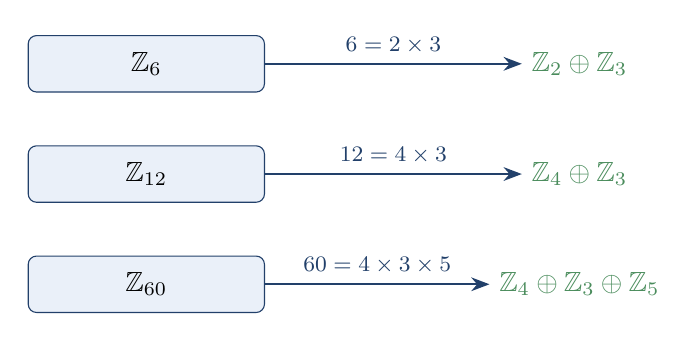
\begin{tikzpicture}[>=Stealth]
  \tikzstyle{mybox}=[draw=SectCol, rounded corners=3pt, fill=ProbBG,
              inner sep=6pt, font=\normalsize, minimum width=3cm]
  \tikzstyle{myres}=[font=\normalsize\bfseries, text=SolFrame]
  \tikzstyle{myarr}=[->,thick,SectCol]
  % Z_6
  \node[mybox] (z6) at (0,0) {$\Z_6$};
  \node[myres] (r6) at (5.5,0) {$\Z_2 \oplus \Z_3$};
  \draw[myarr] (z6) -- node[above,font=\footnotesize]{$6 = 2\times 3$} (r6);
  % Z_12
  \node[mybox] (z12) at (0,-1.4) {$\Z_{12}$};
  \node[myres] (r12) at (5.5,-1.4) {$\Z_4 \oplus \Z_3$};
  \draw[myarr] (z12) -- node[above,font=\footnotesize]{$12 = 4\times 3$} (r12);
  % Z_60
  \node[mybox] (z60) at (0,-2.8) {$\Z_{60}$};
  \node[myres] (r60) at (5.5,-2.8) {$\Z_4 \oplus \Z_3 \oplus \Z_5$};
  \draw[myarr] (z60) -- node[above,font=\footnotesize]{$60 = 4\times 3\times 5$} (r60);
\end{tikzpicture}
\end{center}

\textbf{Նշում.} $\Z_4$-ը հնարավոր չէ հետագայում վերլուծել որպես $\Z_2 \oplus \Z_2$,
քանի որ $\Z_4$-ը ունի 4 կարգի տարր, մինչդեռ $\Z_2 \oplus \Z_2$-ի յուրաքանչյուր տարր
ունի $\leq 2$ կարգ: \qed
\end{sol}

\bigskip
%==========================================================================
\section{\armtext{12 կարգի ոչ ցիկլիկ աբելյան խմբի ենթախմբերը}}
%==========================================================================

\begin{problem}
Քանի՞ 2 և 6 կարգի ենթախումբ ունի 12 կարգի ոչ ցիկլիկ աբելյան խումբը:
\end{problem}

\begin{sol}
12 կարգի ոչ ցիկլիկ աբելյան խումբը $G = \Z_2 \oplus \Z_6 \;\cong\; \Z_2 \oplus \Z_2 \oplus \Z_3$ խումբն է:

\medskip
\textbf{\color{SectCol}2-րդ կարգի ենթախմբեր.}\;
$(a,b) \neq (0,0)$ տարրը ունի 2 կարգ այն և միայն այն դեպքում, երբ $2(a,b)=(0,0)$, այսինքն՝
$b \in \{0,3\}$: 2-րդ կարգի երեք ոչ միավոր տարրերն են՝
$(1,0)$, $(0,3)$, $(1,3)$, որոնցից յուրաքանչյուրը ծնում է տարբեր ենթախումբ:
\[
  \gen{(1,0)},\quad \gen{(0,3)},\quad \gen{(1,3)}.
\]

\medskip
\textbf{\color{SectCol}6-րդ կարգի ենթախմբեր.}\;
Դրանք $\varphi\colon G \to \Z_2$ սյուրյեկտիվ հոմոմորֆիզմների միջուկներն են:
Այդպիսի $\varphi$-ն որոշվում է $\bigl(\varphi(1,0),\, \varphi(0,1)\bigr) \in \Z_2^2$ արժեքներով:
4 հոմոմորֆիզմներից 3-ը սյուրյեկտիվ են (բացառությամբ զրոյականի).

\smallskip
\begin{center}
\renewcommand{\arraystretch}{1.2}
\begin{tabular}{ccc}
  \toprule
  $\varphi(1,0)$ & $\varphi(0,1)$ & $\ker\varphi$ \\
  \midrule
  $1$ & $0$ & $\{0\}\oplus\Z_6 \cong \Z_6$ \\
  $0$ & $1$ & $\Z_2\oplus\{0,2,4\} \cong \Z_2\oplus\Z_3$ \\
  $1$ & $1$ & $\{(0,0),(0,2),(0,4),(1,1),(1,3),(1,5)\} \cong \Z_6$ \\
  \bottomrule
\end{tabular}
\end{center}

\medskip
$G$-ն ունի $\boxed{3}$ ենթախումբ 2 կարգի և $\boxed{3}$ ենթախումբ 6 կարգի: \qed
\end{sol}

\bigskip
%==========================================================================
\section{\armtext{18 կարգի ոչ ցիկլիկ աբելյան խմբի ենթախմբերը}}
%==========================================================================

\begin{problem}
Քանի՞ 3 և 6 կարգի ենթախումբ ունի 18 կարգի ոչ ցիկլիկ աբելյան խումբը:
\end{problem}

\begin{sol}
18 կարգի ոչ ցիկլիկ աբելյան խումբը $G = \Z_3 \oplus \Z_3 \oplus \Z_2$ խումբն է:

\medskip
\textbf{\color{SectCol}3-րդ կարգի ենթախմբեր.}\;
3-րդ կարգի տարրերը պետք է բավարարեն $3(a,b,c) = 0$; քանի որ $\gcd(3,2)=1$, սա
պարտադրում է $c=0$: Ուստի 3-ի բաժանարար կարգ ունեցող տարրերը $(a,b,0)$ տեսքի 9 տարրերն են,
որտեղ $a,b \in \Z_3$: Հեռացնելով միավորը, մնում է ճիշտ 3 կարգի 8 տարր:
Յուրաքանչյուր 3 կարգի ցիկլիկ խումբ պարունակում է 2 այդպիսի տարր,
ուստի ունենք $8/2 = \boxed{4}$ ենթախումբ:
\[
  \gen{(1,0,0)}, \quad \gen{(0,1,0)}, \quad \gen{(1,1,0)}, \quad \gen{(1,2,0)}.
\]

\textbf{\color{SectCol}6-րդ կարգի ենթախմբեր.}\;
Դրանք $\varphi\colon G \to \Z_3$ սյուրյեկցիաների միջուկներն են: Այդպիսի $\varphi$-ն
որոշվում է $\varphi(1,0,0)$ և $\varphi(0,1,0)$ արժեքներով (քանի որ $\gcd(2,3)=1$-ը պարտադրում է
$\varphi(0,0,1)=0$): Ընդհանուր 9 հոմոմորֆիզմներից 8-ը սյուրյեկտիվ են:
Երկու սյուրյեկցիա ունեն նույն միջուկը այն և միայն այն դեպքում, երբ տարբերվում են $\Z_3^* = \{1,2\}$--ի միավորով,
ուստի ստանում ենք $8/2 = \boxed{4}$ ենթախումբ 6 կարգի: \qed
\end{sol}

\bigskip
%==========================================================================
\section{\armtext{200 կարգի աբելյան խմբեր}}
%==========================================================================

\begin{problem}
Նկարագրել 200 կարգի բոլոր աբելյան խմբերը (իզոմորֆիզմի ճշտությամբ):
\end{problem}

\begin{sol}
$200 = 2^3 \times 5^2$: Ըստ հիմնական թեորեմի, մենք անկախորեն տրոհում ենք յուրաքանչյուր
պարզ թվի աստիճանի ցուցիչը:

\begin{center}
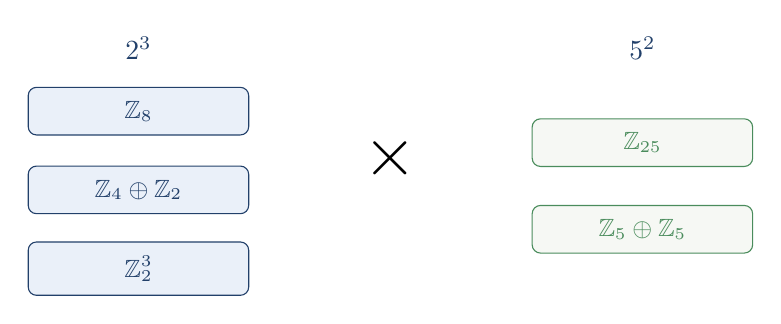
\begin{tikzpicture}[>=Stealth]
  \tikzstyle{partb}=[draw=SectCol, rounded corners=3pt, fill=ProbBG,
               inner sep=5pt, font=\small, text=SectCol, minimum width=2.8cm]
  % 2^3 partitions
  \node[font=\normalsize\bfseries\sffamily, SectCol] at (-3.2,2.4) {$2^3$};
  \node[partb] at (-3.2,1.6) {$\Z_8$};
  \node[partb] at (-3.2,0.6) {$\Z_4\oplus\Z_2$};
  \node[partb] at (-3.2,-0.4) {$\Z_2^3$};
  % 5^2 partitions
  \node[font=\normalsize\bfseries\sffamily, SectCol] at (3.2,2.4) {$5^2$};
  \node[partb, fill=SolBG, draw=SolFrame, text=SolFrame] at (3.2,1.2) {$\Z_{25}$};
  \node[partb, fill=SolBG, draw=SolFrame, text=SolFrame] at (3.2,0.1) {$\Z_5\oplus\Z_5$};
  % cross symbol
  \node[font=\Huge] at (0,1) {$\times$};
\end{tikzpicture}
\end{center}

\smallskip
$3 \times 2 = 6$ ոչ իզոմորֆ խմբերն են.

\begin{center}
\renewcommand{\arraystretch}{1.3}
\begin{tabular}{cl}
  \toprule
  \# & \armtext{Խումբ} \\
  \midrule
  1 & $\Z_8 \oplus \Z_{25} \;\cong\; \Z_{200}$ \\
  2 & $\Z_8 \oplus \Z_5 \oplus \Z_5$ \\
  3 & $\Z_4 \oplus \Z_2 \oplus \Z_{25}$ \\
  4 & $\Z_4 \oplus \Z_2 \oplus \Z_5 \oplus \Z_5$ \\
  5 & $\Z_2 \oplus \Z_2 \oplus \Z_2 \oplus \Z_{25}$ \\
  6 & $\Z_2 \oplus \Z_2 \oplus \Z_2 \oplus \Z_5 \oplus \Z_5$ \\
  \bottomrule
\end{tabular}
\end{center}

Գոյություն ունի $\boxed{6}$ ոչ իզոմորֆ 200 կարգի աբելյան խումբ: \qed
\end{sol}

\bigskip
%==========================================================================
\section{\armtext{$\Z_3 \oplus \Z_3$ խմբի բոլոր ենթախմբերը}}
%==========================================================================

\begin{problem}
Գտնել $\Z_3 \oplus \Z_3$ խմբի բոլոր ենթախմբերը:
\end{problem}

\begin{sol}
$G = \Z_3 \oplus \Z_3$ խումբը ունի 9 տարր: Հնարավոր ենթախմբերի կարգերն են՝ $1, 3, 9$:

\medskip
\textbf{\color{SectCol}Կարգ 1:} $\{(0,0)\}$:
\qquad\textbf{\color{SectCol}Կարգ 9:} $G$-ն ինքը:

\medskip
\textbf{\color{SectCol}Կարգ 3:}
8 ոչ միավոր տարրերը զույգվում են ($g$-ն և $2g$-ն ծնում են նույն ենթախումբը),
տալով $8/2 = 4$ ցիկլիկ ենթախումբ.

\smallskip
\begin{center}
\renewcommand{\arraystretch}{1.15}
\begin{tabular}{cl}
  \toprule
  \armtext{Ենթախումբ} & \armtext{Տարրեր} \\
  \midrule
  $H_1 = \gen{(1,0)}$ & $\{(0,0),\,(1,0),\,(2,0)\}$ \\
  $H_2 = \gen{(0,1)}$ & $\{(0,0),\,(0,1),\,(0,2)\}$ \\
  $H_3 = \gen{(1,1)}$ & $\{(0,0),\,(1,1),\,(2,2)\}$ \\
  $H_4 = \gen{(1,2)}$ & $\{(0,0),\,(1,2),\,(2,1)\}$ \\
  \bottomrule
\end{tabular}
\end{center}

\medskip
Ընդհանուր առմամբ, $\Z_3 \oplus \Z_3$-ն ունի ճիշտ $\boxed{6}$ ենթախումբ:
\end{sol}

\medskip
\begin{center}
\begin{tikzpicture}[scale=1]
  % --- Left: lattice diagram ---
  \node[font=\small\bfseries\sffamily,SectCol] at (-4,4.2) {\armtext{Ենթախմբերի ցանց}};
  \node[draw,rounded corners=3pt,fill=ProbFrame!15,inner sep=4pt,font=\small]
    (top) at (-4,3.5) {$\Z_3\oplus\Z_3$};
  \node[draw,rounded corners=3pt,fill=ProbBG,inner sep=3pt,font=\scriptsize]
    (a) at (-6.4,1.75) {$\gen{(1,0)}$};
  \node[draw,rounded corners=3pt,fill=ProbBG,inner sep=3pt,font=\scriptsize]
    (b) at (-4.8,1.75) {$\gen{(0,1)}$};
  \node[draw,rounded corners=3pt,fill=ProbBG,inner sep=3pt,font=\scriptsize]
    (c) at (-3.2,1.75) {$\gen{(1,1)}$};
  \node[draw,rounded corners=3pt,fill=ProbBG,inner sep=3pt,font=\scriptsize]
    (d) at (-1.6,1.75) {$\gen{(1,2)}$};
  \node[draw,rounded corners=3pt,fill=SolBG,inner sep=4pt,font=\small]
    (bot) at (-4,0) {$\{(0,0)\}$};
  \draw[thick,ProbFrame] (top)--(a)--(bot) (top)--(b)--(bot)
                         (top)--(c)--(bot) (top)--(d)--(bot);

  % --- Right: grid of Z_3 x Z_3 elements ---
  \node[font=\small\bfseries\sffamily,SectCol] at (4.5,4.2)
    {\armtext{$\Z_3\oplus\Z_3$-ի տարրերը}};
  \draw[step=1,GridGray,thin] (3,-0.5) grid (6.5,2.5);
  \draw[->,thick,gray!60] (3,0)--(7,0) node[right,font=\tiny]{$a$};
  \draw[->,thick,gray!60] (3.5,-0.5)--(3.5,3) node[above,font=\tiny]{$b$};
  % H1: along a-axis (blue)
  \fill[ProbFrame]    (3.5,0) circle (5pt);
  \fill[ProbFrame!70] (4.5,0) circle (4pt);
  \fill[ProbFrame!70] (5.5,0) circle (4pt);
  % H2: along b-axis (green)
  \fill[SolFrame!70]  (3.5,1) circle (4pt);
  \fill[SolFrame!70]  (3.5,2) circle (4pt);
  % H3: diagonal (gold)
  \fill[AccGold]      (4.5,1) circle (4pt);
  \fill[AccGold]      (5.5,2) circle (4pt);
  % H4: anti-diagonal (red)
  \fill[red!60!black] (4.5,2) circle (4pt);
  \fill[red!60!black] (5.5,1) circle (4pt);
  % element labels
  \node[font=\tiny,above right,inner sep=1pt] at (3.58,0.08) {$(0,0)$};
  \node[font=\tiny,above right,inner sep=1pt] at (4.58,0.08) {$(1,0)$};
  \node[font=\tiny,above right,inner sep=1pt] at (5.58,0.08) {$(2,0)$};
  \node[font=\tiny,above right,inner sep=1pt] at (3.58,1.08) {$(0,1)$};
  \node[font=\tiny,above right,inner sep=1pt] at (4.58,1.08) {$(1,1)$};
  \node[font=\tiny,above right,inner sep=1pt] at (5.58,1.08) {$(2,1)$};
  \node[font=\tiny,above right,inner sep=1pt] at (3.58,2.08) {$(0,2)$};
  \node[font=\tiny,above right,inner sep=1pt] at (4.58,2.08) {$(1,2)$};
  \node[font=\tiny,above right,inner sep=1pt] at (5.58,2.08) {$(2,2)$};
  % legend
  \fill[ProbFrame]    (6.65,2.3) circle (3pt);
  \node[font=\tiny,ProbFrame,    right] at (6.85,2.3) {$H_1$};
  \fill[SolFrame]     (6.65,1.8) circle (3pt);
  \node[font=\tiny,SolFrame,     right] at (6.85,1.8) {$H_2$};
  \fill[AccGold]      (6.65,1.3) circle (3pt);
  \node[font=\tiny,AccGold,      right] at (6.85,1.3) {$H_3$};
  \fill[red!60!black] (6.65,0.8) circle (3pt);
  \node[font=\tiny,red!60!black, right] at (6.85,0.8) {$H_4$};
\end{tikzpicture}
\end{center}

\smallskip
\noindent \armtext{Ցանցն ունի բնութագրական \emph{շեղանկյուն} տեսք ($M_4$): Յուրաքանչյուր 3 կարգի
զույգ տարբեր ենթախմբեր հատվում են միայն միավորով և միասին ծնում են ամբողջ խումբը:}

\end{document}
